\documentclass{beamer}
\usepackage{listings}
\lstset{
%language=C,
frame=single, 
breaklines=true,
columns=fullflexible
}
\usepackage{gensymb}
\usepackage{subcaption}
\usepackage{url}
\usepackage{tikz}
\usepackage{tkz-euclide} % loads  TikZ and tkz-base
%\usetkzobj{all}
\usetikzlibrary{calc,math}
\usepackage{float}
\newcommand{\myvec}[1]{\ensuremath{\begin{pmatrix}#1\end{pmatrix}}}
\providecommand{\brak}[1]{\ensuremath{\left(#1\right)}}
\newcommand\norm[1]{\left\lVert#1\right\rVert}
\renewcommand{\vec}[1]{\mathbf{#1}}
\providecommand{\abs}[1]{\vert#1\vert}
\usepackage[export]{adjustbox}
\usepackage[utf8]{inputenc}
\usepackage{amsmath}
\newtheorem*{remark}{Remark}
\providecommand{\mbf}{\mathbf}
\providecommand{\pr}[1]{\ensuremath{\Pr\left(#1\right)}}
\providecommand{\qfunc}[1]{\ensuremath{Q\left(#1\right)}}
\providecommand{\sbrak}[1]{\ensuremath{{}\left[#1\right]}}
\providecommand{\lsbrak}[1]{\ensuremath{{}\left[#1\right.}}
\providecommand{\rsbrak}[1]{\ensuremath{{}\left.#1\right]}}
\providecommand{\brak}[1]{\ensuremath{\left(#1\right)}}
\providecommand{\lbrak}[1]{\ensuremath{\left(#1\right.}}
\providecommand{\rbrak}[1]{\ensuremath{\left.#1\right)}}
\providecommand{\cbrak}[1]{\ensuremath{\left\{#1\right\}}}
\providecommand{\lcbrak}[1]{\ensuremath{\left\{#1\right.}}
\providecommand{\rcbrak}[1]{\ensuremath{\left.#1\right\}}}
\usetheme{Boadilla}
\providecommand{\pr}[1]{\ensuremath{\Pr\left(#1\right)}}

\title{Gate Assignment 1 Presentation}
\author{Yashas Tadikamalla}
\date{AI20BTECH11027}
\begin{document}

\begin{frame}
\titlepage
\end{frame}
\begin{frame}
\frametitle{Question}
\begin{block}{Problem (EC-2013 Q8)}
The impulse response of a system is $h(t)=tu(t)$. For an input $u(t-1)$, the output is 
\begin{enumerate}
    \item $\dfrac{t^{2}}{2}u(t)$
    \item $\dfrac{t(t-1)}{2}u(t-1)$
    \item $\dfrac{(t-1)^{2}}{2}u(t-1)$
    \item $\dfrac{t^{2}-1}{2}u(t-1)$
\end{enumerate}
\end{block}
\end{frame}

\begin{frame}
\frametitle{Few prerequisites}
\begin{definition}[Laplace Transform]
It is an integral transform that converts a function of a real variable $t$ to a function of a complex variable $s$. The Laplace transform of $f(t)$ is denoted by $\mathcal{L}\cbrak{f(t)}$ or $F(s)$.
\begin{align}
    F(s)=\mathcal{L}\cbrak{f(t)}=\int_{0}^{\infty}e^{-st}f(t)dt
\end{align}
\end{definition}
\begin{remark}
Laplace transform of $f(t)=t^n,n\geq1$ is
\begin{align}
    F(s)=\mathcal{L}\cbrak{t^n}=\dfrac{n!}{s^{n+1}},Re(s)>0
    \label{eq:t}
\end{align}
\end{remark}
\end{frame}


\begin{frame}
\frametitle{}
\begin{block}{Proof.}
Basis Step: $n=1$
\begin{align}
    \mathcal{L}\cbrak{t}&=\int_{0}^{\infty}e^{-st}tdt=\sbrak{\dfrac{te^{-st}}{-s}}_{0}^{\infty}+\dfrac{1}{s}\int_{0}^{\infty}e^{-st}dt\\
    &=0+\sbrak{\dfrac{-1}{s^2}e^{-st}}_{0}^{\infty},Re(s)>0=\dfrac{1}{s^2},Re(s)>0
\end{align}
Inductive Step:
\begin{align}
    \mathcal{L}\cbrak{t^n}&=\int_{0}^{\infty}e^{-st}t^ndt=\sbrak{\dfrac{t^{n}e^{-st}}{-s}}_{0}^{\infty}+\dfrac{n}{s}\int_{0}^{\infty}t^{n-1}e^{-st}dt\\
    &=0+\dfrac{n}{s}\mathcal{L}\cbrak{t^{n-1}},Re(s)>0=\dfrac{n}{s}\mathcal{L}\cbrak{t^{n-1}},Re(s)>0\label{eq:e}
\end{align}
\end{block}
\end{frame}

\begin{frame}
\frametitle{}
\begin{proof}
To prove that if \eqref{eq:t} holds for $n=k$, it holds for $n=k+1$. From \eqref{eq:e}
\begin{align}
    \mathcal{L}\cbrak{t^{k+1}}&=\dfrac{k+1}{s}\mathcal{L}\cbrak{t^{k}}\\
    &=\dfrac{(k+1)k!}{s(s^{k+1})}=\dfrac{(k+1)!}{s^{k+2}}, Re(s)>0
\end{align}
By mathematical induction, \eqref{eq:t} is true $\forall n\geq 1$
\end{proof}
\begin{lemma}
For any real number c, 
\begin{align}
    \mathcal{L}\cbrak{u(t-c)}=\dfrac{e^{-cs}}{s}, Re(s)>0
    \label{eq:u}
\end{align}
\end{lemma}
\end{frame}

\begin{frame}
\frametitle{}
\begin{proof}
 \begin{align}
     \mathcal{L}\cbrak{u(t-c)}&=\int_{0}^{\infty}e^{-st}u(t-c)dt=\int_{c}^{\infty}e^{-st}dt\\
     &=\sbrak{-\dfrac{e^{-st}}{s}}_{c}^{\infty}=\dfrac{e^{-cs}}{s}, Re(s)>0
 \end{align}
\end{proof}
\begin{definition}[Inverse Laplace Transform]
Its the transformation of a Laplace transform into a function of time. If $F(s)=\mathcal{L}\cbrak{f(t)}$, then Inverse laplace transform of $F(s)$ is $\mathcal{L}^{-1}\cbrak{F(s)}=f(t)$.
\end{definition}
\begin{lemma}[t-shift rule]
For any real number c,
\begin{align}
    \mathcal{L}\cbrak{u(t-c)f(t-c)}=e^{-cs}F(s)
    \label{eq:uf}
\end{align}
\end{lemma}
\end{frame}

\begin{frame}
\frametitle{}
\begin{proof}
\begin{align}
    \mathcal{L}\cbrak{u(t-c)f(t-c)}&=\int_{0}^{\infty}e^{-st}u(t-c)f(t-c)dt\\
    &=\int_{c}^{\infty}e^{-st}f(t-c)dt\\
    &=\int_{0}^{\infty}e^{-s(\tau+c)}f(\tau)d\tau \brak{t=\tau+c}\\
    &=e^{-cs}\int_{0}^{\infty}e^{-s\tau}f(\tau)d\tau=e^{-cs}F(s)
\end{align}
\end{proof}
\begin{corollary}
\begin{align}
    \mathcal{L}^{-1}\cbrak{e^{-cs}F(s)}=u(t-c)f(t-c)
\end{align}
\end{corollary}
\end{frame}

\begin{frame}
\frametitle{}
\begin{theorem}[Convolution theorem]
Suppose $F(s)=\mathcal{L}\cbrak{f(t)}, G(s)=\mathcal{L}\cbrak{g(t)}$ exist, then,
\begin{align}
    \mathcal{L}^{-1}\cbrak{F(s)G(s)}=f(t)*g(t)\label{eq:cuf}
\end{align}
\end{theorem}
\end{frame}


\begin{frame}
\frametitle{Solution}
Given,
\begin{align}
    &h(t)=tu(t)\\
    &x(t)=u(t-1)
\end{align}
To find: $y(t)$. We know, 
\begin{align}
y(t)&=h(t)*x(t)\\
&=\mathcal{L}^{-1}\cbrak{H(s)X(s)}
\label{eq:def}
\end{align}
From \eqref{eq:uf} and \eqref{eq:t}, 
\begin{align}
H(s)=e^{0}\mathcal{L}\cbrak{t}=\dfrac{1}{s^2}
\end{align}
From \eqref{eq:u}, 
\begin{align}
X(s)=\dfrac{e^{-s}}{s}
\end{align}
\end{frame}

\begin{frame}
\frametitle{Solution Contd.}
Substituting in \eqref{eq:def},
\begin{align}
y(t)=\mathcal{L}^{-1}\cbrak{\dfrac{e^{-s}}{s^3}}
\end{align}
Consider 
\begin{align}
    p(t)=\dfrac{t^{2}}{2}
\end{align}
From \eqref{eq:t}
\begin{align}
    P(s)=\dfrac{2!}{2s^3}=\dfrac{1}{s^3}
\end{align}
Further, from \eqref{eq:cuf}, for $c=1$
\begin{align}
    \mathcal{L}^{-1}\cbrak{e^{-s}P(s)}&=u(t-1)p(t-1)=u(t-1)\dfrac{(t-1)^2}{2}\\
    \therefore y(t)&=\dfrac{(t-1)^2}{2}u(t-1)
\end{align}
Option 3 is the correct answer.
\end{frame}

\begin{frame}
\frametitle{Solution Contd.}
\begin{align}
    h(t)&=\begin{cases}
	t, & t \geq 0 \\~\\[-1em]
	0, & t <0
	\end{cases}\\
	x(t)&=\begin{cases}
	1, & t \geq 1 \\~\\[-1em]
	0, & t <1
	\end{cases}\\
	y(t)&=\begin{cases}
	\dfrac{(t-1)^2}{2}, & t \geq 1 \\~\\[-1em]
	0, & t <1
	\end{cases}
\end{align}
\end{frame}

\begin{frame}
\frametitle{Solution Contd.}
\begin{figure}[!h]
 \centering
 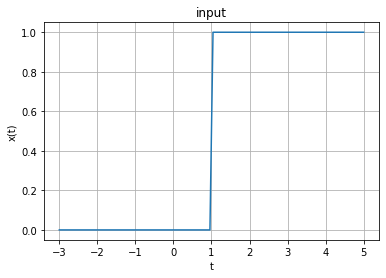
\includegraphics[width=0.75\columnwidth]{GateAssignment1Presentation(1).png}
 \caption{Plot of $x(t)$}
 \label{plot}
\end{figure}
\end{frame}


\begin{frame}
\frametitle{Solution Contd.}
\begin{figure}[!h]
 \centering
 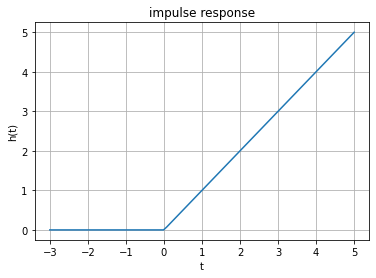
\includegraphics[width=0.75\columnwidth]{GateAssignment1Presentation(2).png}
 \caption{Plot of $h(t)$}
 \label{plot}
\end{figure}
\end{frame}

\begin{frame}
\frametitle{Solution Contd.}
\begin{figure}[!h]
 \centering
 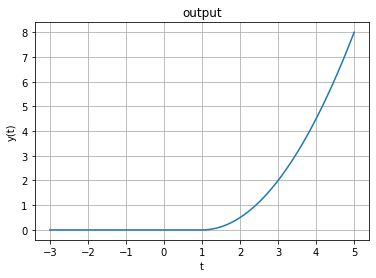
\includegraphics[width=0.75\columnwidth]{GateAssignment1Presentation(3).png}
 \caption{Plot of $y(t)$}
 \label{plot}
\end{figure}
\end{frame}
\end{document}
